\chapter{Applying Rapid Whole-Genome Sequencing To Predict Phenotypic Antimicrobial Susceptibility Testing Results among Carbapenem-Resistant \textit{Klebsiella pneumoniae} Clinical Isolates}
\label{chap:amr}

\textbf{Portions of this chapter originally appeared in:} \\
Tamma PD, Fan Y, Bergman Y, Pertea G, Kazmi AQ, Lewis S, et al. Applying Rapid Whole-Genome Sequencing To Predict Phenotypic Antimicrobial Susceptibility Testing Results among Carbapenem-Resistant \textit{Klebsiella pneumoniae} Clinical Isolates 2019;63. https://doi.org/10.1128/AAC.01923-18

\section{Abstract}
\label{sec:abstract}

Standard antimicrobial susceptibility testing (AST) approaches lead to delays in the selection of optimal antimicrobial therapy. Here, we sought to determine the accuracy of antimicrobial resistance (AMR) determinants identified by Nanopore whole-genome sequencing in predicting AST results. Using a cohort of 40 clinical isolates (21 carbapenemase-producing carbapenem-resistant Klebsiella pneumoniae, 10 non-carbapenemase-producing carbapenem-resistant K. pneumoniae, and 9 carbapenem-susceptible K. pneumoniae isolates), three separate sequencing and analysis pipelines were performed, as follows: (i) a real-time Nanopore analysis approach identifying acquired AMR genes, (ii) an assembly-based Nanopore approach identifying acquired AMR genes and chromosomal mutations, and (iii) an approach using short-read correction of Nanopore assemblies. The short-read correction of Nanopore assemblies served as the reference standard to determine the accuracy of Nanopore sequencing results. With the real-time analysis approach, full annotation of acquired AMR genes occurred within 8 h from subcultured isolates. Assemblies sufficient for full resistance gene and single-nucleotide polymorphism annotation were available within 14 h from subcultured isolates. The overall agreement of genotypic results and anticipated AST results for the 40 K. pneumoniae isolates was 77% (range, 30% to 100%) and 92% (range, 80% to 100%) for the real-time approach and the assembly approach, respectively. Evaluating the patients contributing the 40 isolates, the real-time approach and assembly approach could shorten the median time to effective antibiotic therapy by 20 h and 26 h, respectively, compared to standard AST. Nanopore sequencing offers a rapid approach to both accurately identify resistance mechanisms and to predict AST results for K. pneumoniae isolates. Bioinformatics improvements enabling real-time alignment, coupled with rapid extraction and library preparation, will further enhance the accuracy and workflow of the Nanopore real-time approach.

\section{Introduction}
\label{sec:intro}


\section{Results}
\label{sec:results}

\subsection{Genome statistics}
\label{sec:genstat}




\begin{figure}[!hb]
\centering
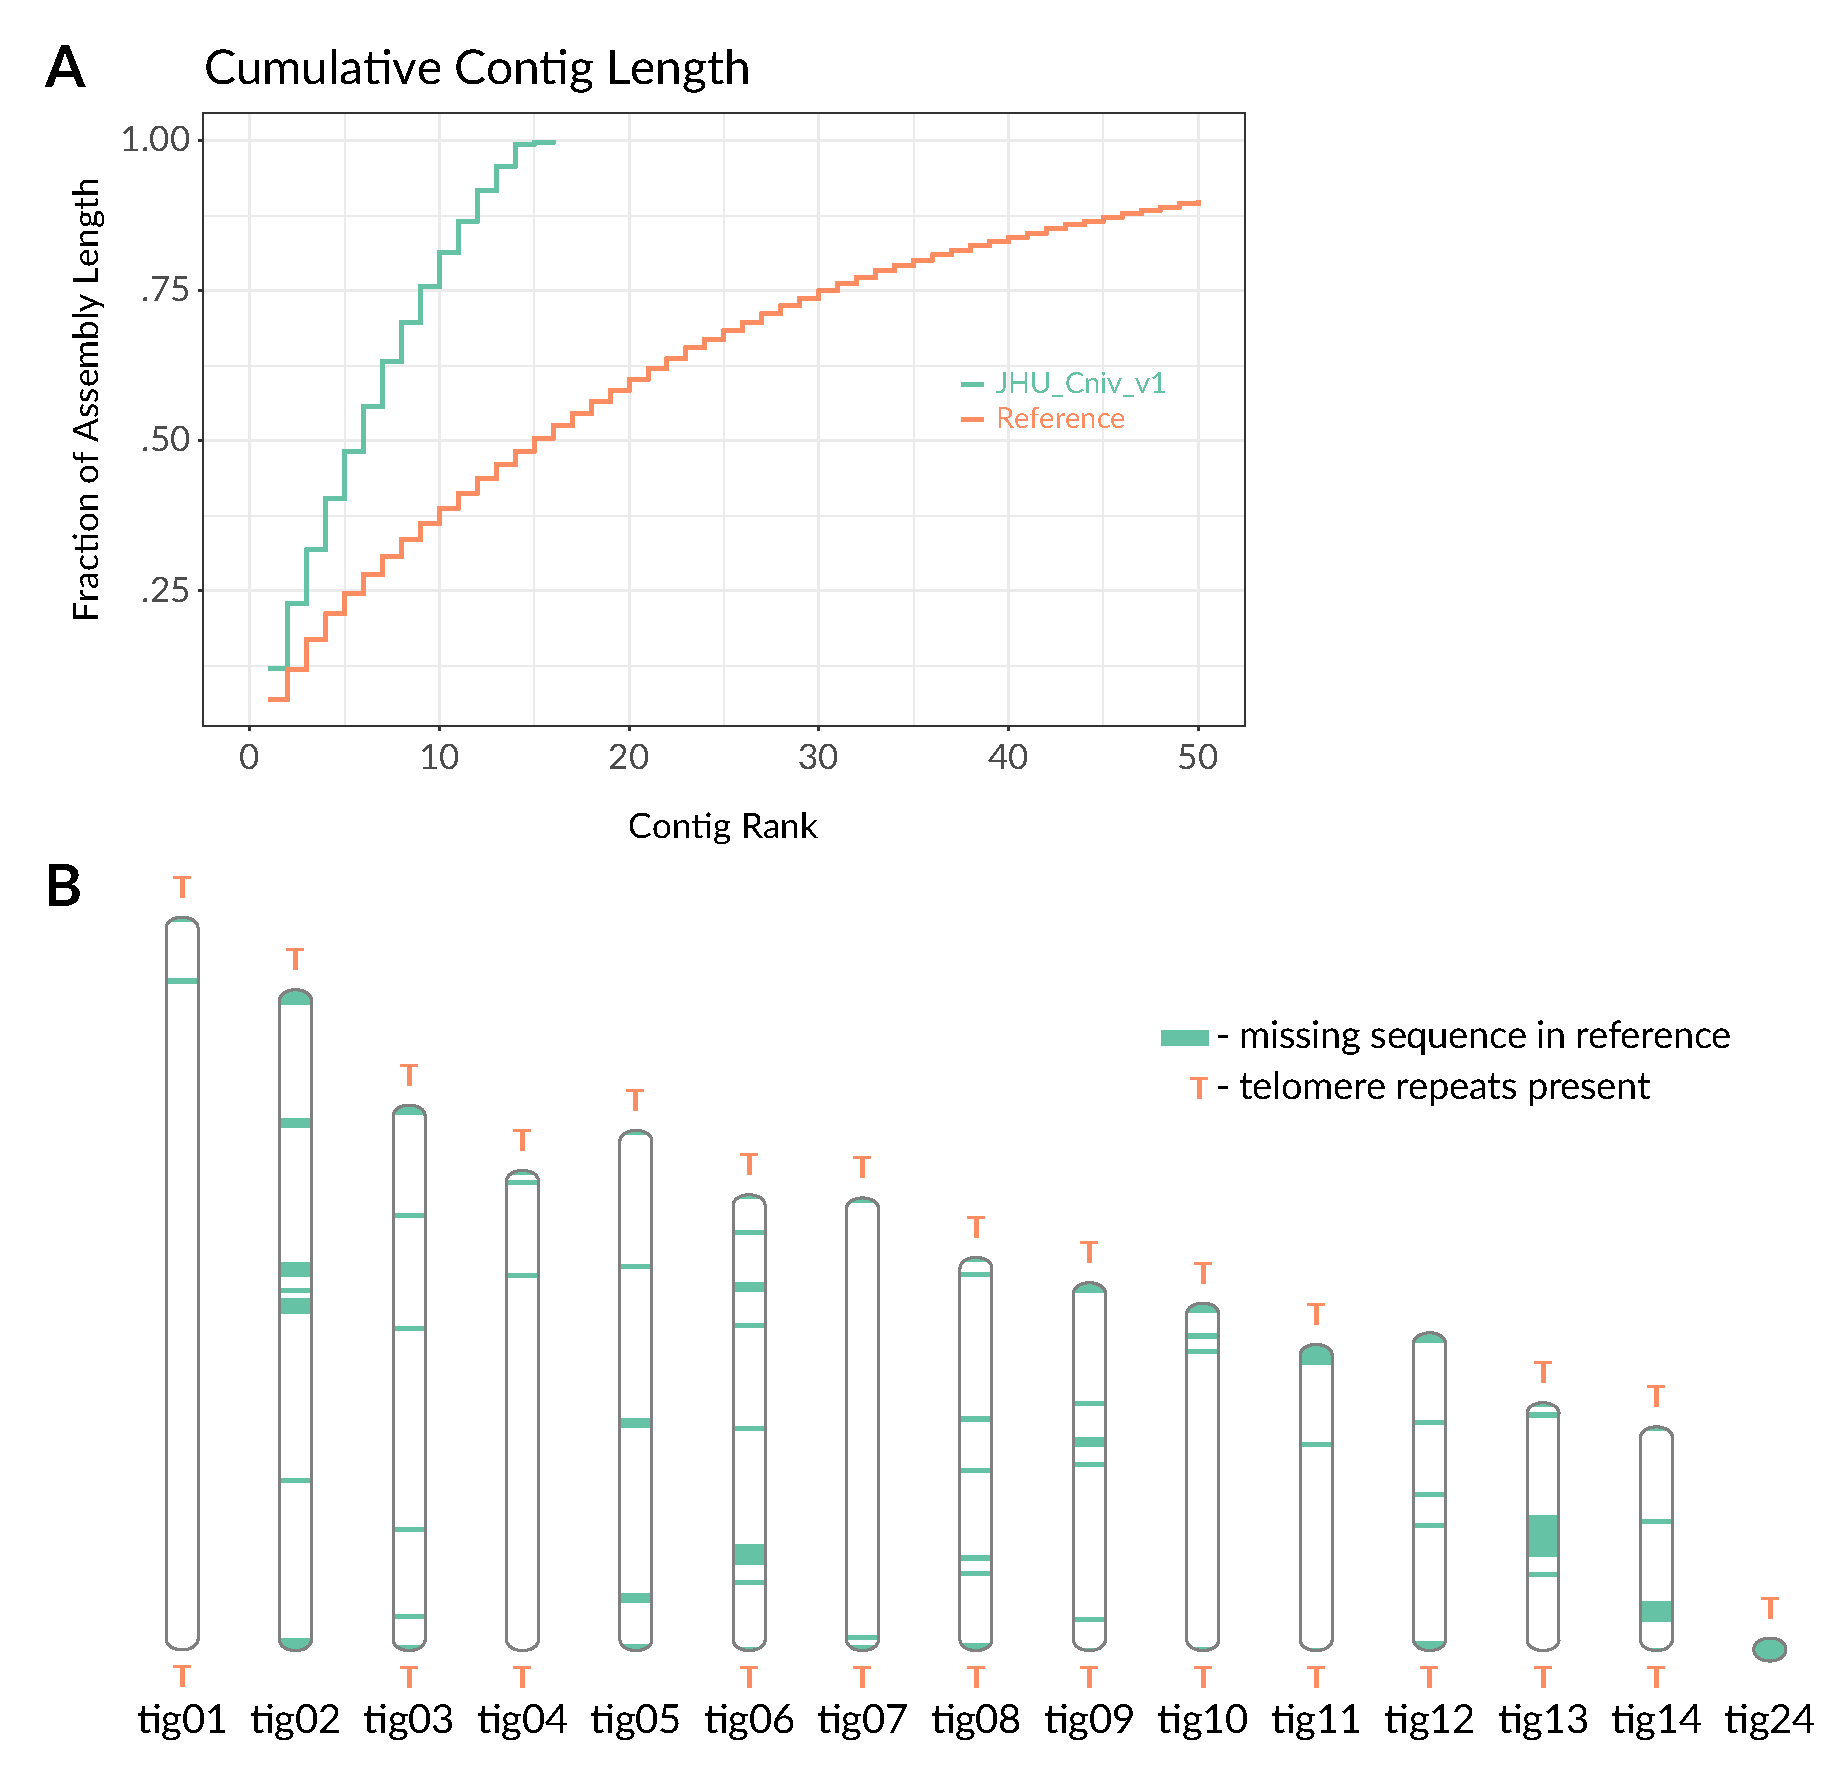
\includegraphics[width = 1\linewidth,keepaspectratio]{figure/asms.pdf}
\caption[Characteristics of the JHU\_Cniv\_v1 assembly]{{\bf Characteristics of the JHU\_Cniv\_v1 assembly.} {\bf (A)} Cumulative lengths of the 50 longest sequences in our assembly and previous reference genome. {\bf (B)} Ideogram of assembly. Sequence that is missing in the reference genome is shown along each non-mitochondrial contig, and the positions of telomere repeats are marked. }
\label{fig:asms}
\end{figure}


\begin{table}[!hb]
\centering
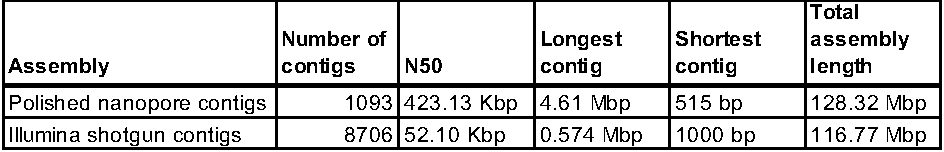
\includegraphics[width = 1\linewidth,keepaspectratio]{figure/asmstats.pdf}
\caption[Assembly Statistics]{{\bf Assembly Statistics.} Assembly statistics of JHU\_Cniv\_v1 and the reference genome for \textit{C. nivariensis}. }
\label{tab:asmstats}
\end{table}



\subsection{Genome completeness}
\label{sec:gencomp}


\subsection{Repetitive genes}
\label{sec:repgenes}





\section{Discussion}
\label{sec:discuss}




\section{Methods}
\label{sec:methods}

\subsection{Media and growth conditions}
\label{sec:methods}



\subsection{DNA isolation and sequencing}
\label{sec:methods}


\subsection{RNA isolation and sequencing}
\label{sec:methods}


\subsection{Genome assembly}
\label{sec:methods}




\subsection{Annotation}
\label{sec:methods}



\subsection{Data Availability}
\label{sec:methods}
